\documentclass{beamer}
\usepackage[utf8]{inputenc}

\usetheme{Madrid}
\usecolortheme{default}
\usepackage{amsmath}
\usepackage{amssymb,amsfonts,amsthm}
\usepackage{txfonts}
\usepackage{tkz-euclide}
\usepackage{listings}
\usepackage{adjustbox}
\usepackage{array}
\usepackage{tabularx}
\usepackage{gvv}
\usepackage{lmodern}
\usepackage{circuitikz}
\usepackage{tikz}
\usepackage{graphicx}

\setbeamertemplate{page number in head/foot}[totalframenumber]

\usepackage{tcolorbox}
\tcbuselibrary{minted,breakable,xparse,skins}



\definecolor{bg}{gray}{0.95}
\DeclareTCBListing{mintedbox}{O{}m!O{}}{%
  breakable=true,
  listing engine=minted,
  listing only,
  minted language=#2,
  minted style=default,
  minted options={%
    linenos,
    gobble=0,
    breaklines=true,
    breakafter=,,
    fontsize=\small,
    numbersep=8pt,
    #1},
  boxsep=0pt,
  left skip=0pt,
  right skip=0pt,
  left=25pt,
  right=0pt,
  top=3pt,
  bottom=3pt,
  arc=5pt,
  leftrule=0pt,
  rightrule=0pt,
  bottomrule=2pt,
  toprule=2pt,
  colback=bg,
  colframe=orange!70,
  enhanced,
  overlay={%
    \begin{tcbclipinterior}
    \fill[orange!20!white] (frame.south west) rectangle ([xshift=20pt]frame.north west);
    \end{tcbclipinterior}},
  #3,
}
\lstset{
    language=C,
    basicstyle=\ttfamily\small,
    keywordstyle=\color{blue},
    stringstyle=\color{orange},
    commentstyle=\color{green!60!black},
    numbers=left,
    numberstyle=\tiny\color{gray},
    breaklines=true,
    showstringspaces=false,
}

% Custom math commands

% Metadata
\title{Matgeo Presentation- problem 1.5.9}
\author{Dhanush sagar}
\institute{IIT Hyderabad}
\date{\today}

% Beamer templates
\setbeamertemplate{footline}[frame number]
\setbeamertemplate{navigation symbols}{}

\begin{document}

\begin{frame}
  \titlepage
\end{frame}

\begin{frame}{Outline}
  \tableofcontents
\end{frame}

% ==================
\section{Problem statement}
\begin{frame}{Question}
We are given two points 
\[ A(5,-6), \quad B(-1,-4). \]
The point $P$ divides $AB$ in the ratio $5:1$. We need to find $P$ and plot all three points with the line.
\end{frame}


\begin{frame}{Solution}
given points are A and B
\begin{align*} \vec{A} = \myvec{5 \\ -6}, \vec{B} = \myvec{-1 \\ -4} \end{align*}
Let the Y-axis divide the \(\overline{\vec{AB}}\) at point $\vec{P}$ in the ratio $k:1$.
Since $\vec{P}$ lies on Y-axis, let intersection point P be
\begin{align*}
\vec{P} = \myvec{0 \\ y}
\end{align*}
The point $\vec{A}$, $\vec{B}$, $\vec{P}$ are collinear.
\begin{align}
\implies \text{rank}\myvec{\vec{B}-\vec{A} & \vec{P}-\vec{A}} = 1
\end{align}
\begin{align}
\myvec{-6 & -5 \\ 2 & y+6} \xleftrightarrow[]{R_2 \rightarrow {\frac{1}{3}R_1 + R_2}}\myvec{-6 & -5 \\ 0 & y+\frac{13}{3}}  
\end{align}

\end{frame}


\begin{frame}{Solution}
The number of nonzero rows in the row reduced matrix is defined as the rank. For above matrix to be of rank 1,
\begin{align}
y+\frac{13}{3} &= 0 \\
y &= \frac{-13}{3}
\end{align}
$\therefore$ The coordinates of the point of intersection are 
\begin{align*}
\vec{P} = \myvec{0 \\ \frac{-13}{3}}
\end{align*}

Substituting the values of $\vec{A}$, $\vec{B}$ and $\vec{P}$,
\begin{align}
k=\frac{\myvec{5 & \frac{-5}{3}}\myvec{1 \\ \frac{-1}{3}}}{\norm{\myvec{1 \\ \frac{-1}{3}}}^2}=5
\end{align}
\end{frame}
% ==================
\section{C Code}
\begin{frame}[fragile]{main.c}
\begin{lstlisting}[language=C]
#include <stdio.h>
int main() {
    FILE *fp = fopen("points.dat", "w");
    if (fp == NULL) return 1;
    fprintf(fp, "5 -6\n");
    fprintf(fp, "-1 -4\n");
    fprintf(fp, "0 -4.3333\n");
    fclose(fp);
    return 0;
}
\end{lstlisting}
\end{frame}

\begin{frame}[fragile]{write\_points.c}
\begin{lstlisting}[language=C]
#include <stdio.h>
int main() {
    FILE *fp = fopen("points.dat", "w");
    if (fp == NULL) return 1;
    fprintf(fp, "5 -6\n");
    fprintf(fp, "-1 -4\n");
    fprintf(fp, "0 -13/3\n");
    fclose(fp);
    return 0;
}
\end{lstlisting}
\end{frame}

% ==================
\section{Python Code}
\begin{frame}[fragile]{plot\_points.py}
\begin{lstlisting}[language=Python]
import numpy as np
import matplotlib.pyplot as plt

# Load points from file
data = np.loadtxt('points.dat')

x, y = data[:,0], data[:,1]

plt.plot(x, y, 'bo--', label='Line through A, P, B')
plt.scatter(5,-6,color='red',label='A(5,-6)')
plt.scatter(-1,-4,color='green',label='B(-1,-4)')
plt.scatter(0,-13/3,color='purple',label='P(0,-13/3)')

plt.axvline(0, color='gray', linestyle='--')
plt.xlabel('X-axis')
plt.ylabel('Y-axis')
plt.title('Points and Line Division (Ratio 5:1)')
plt.legend()
plt.grid(True)
plt.show()
\end{lstlisting}
\end{frame}

% ==================
\section{Data File}
\begin{frame}[fragile]{points.dat}
\begin{lstlisting}
5 -6
-1 -4
0 -4.3333
\end{lstlisting}
\end{frame}

\begin{frame}{Points Table}
\centering
\begin{tabular}{|c|c|c|}
\hline
Point & x & y \\
\hline
A & 5 & -6 \\
B & -1 & -4 \\
P & 0 & $-\tfrac{13}{3}$ \\
\hline
\end{tabular}
\end{frame}

% ==================
\section{Plot Result}
\begin{frame}{Graphical Output}
 \begin{figure}[H]
     \centering
     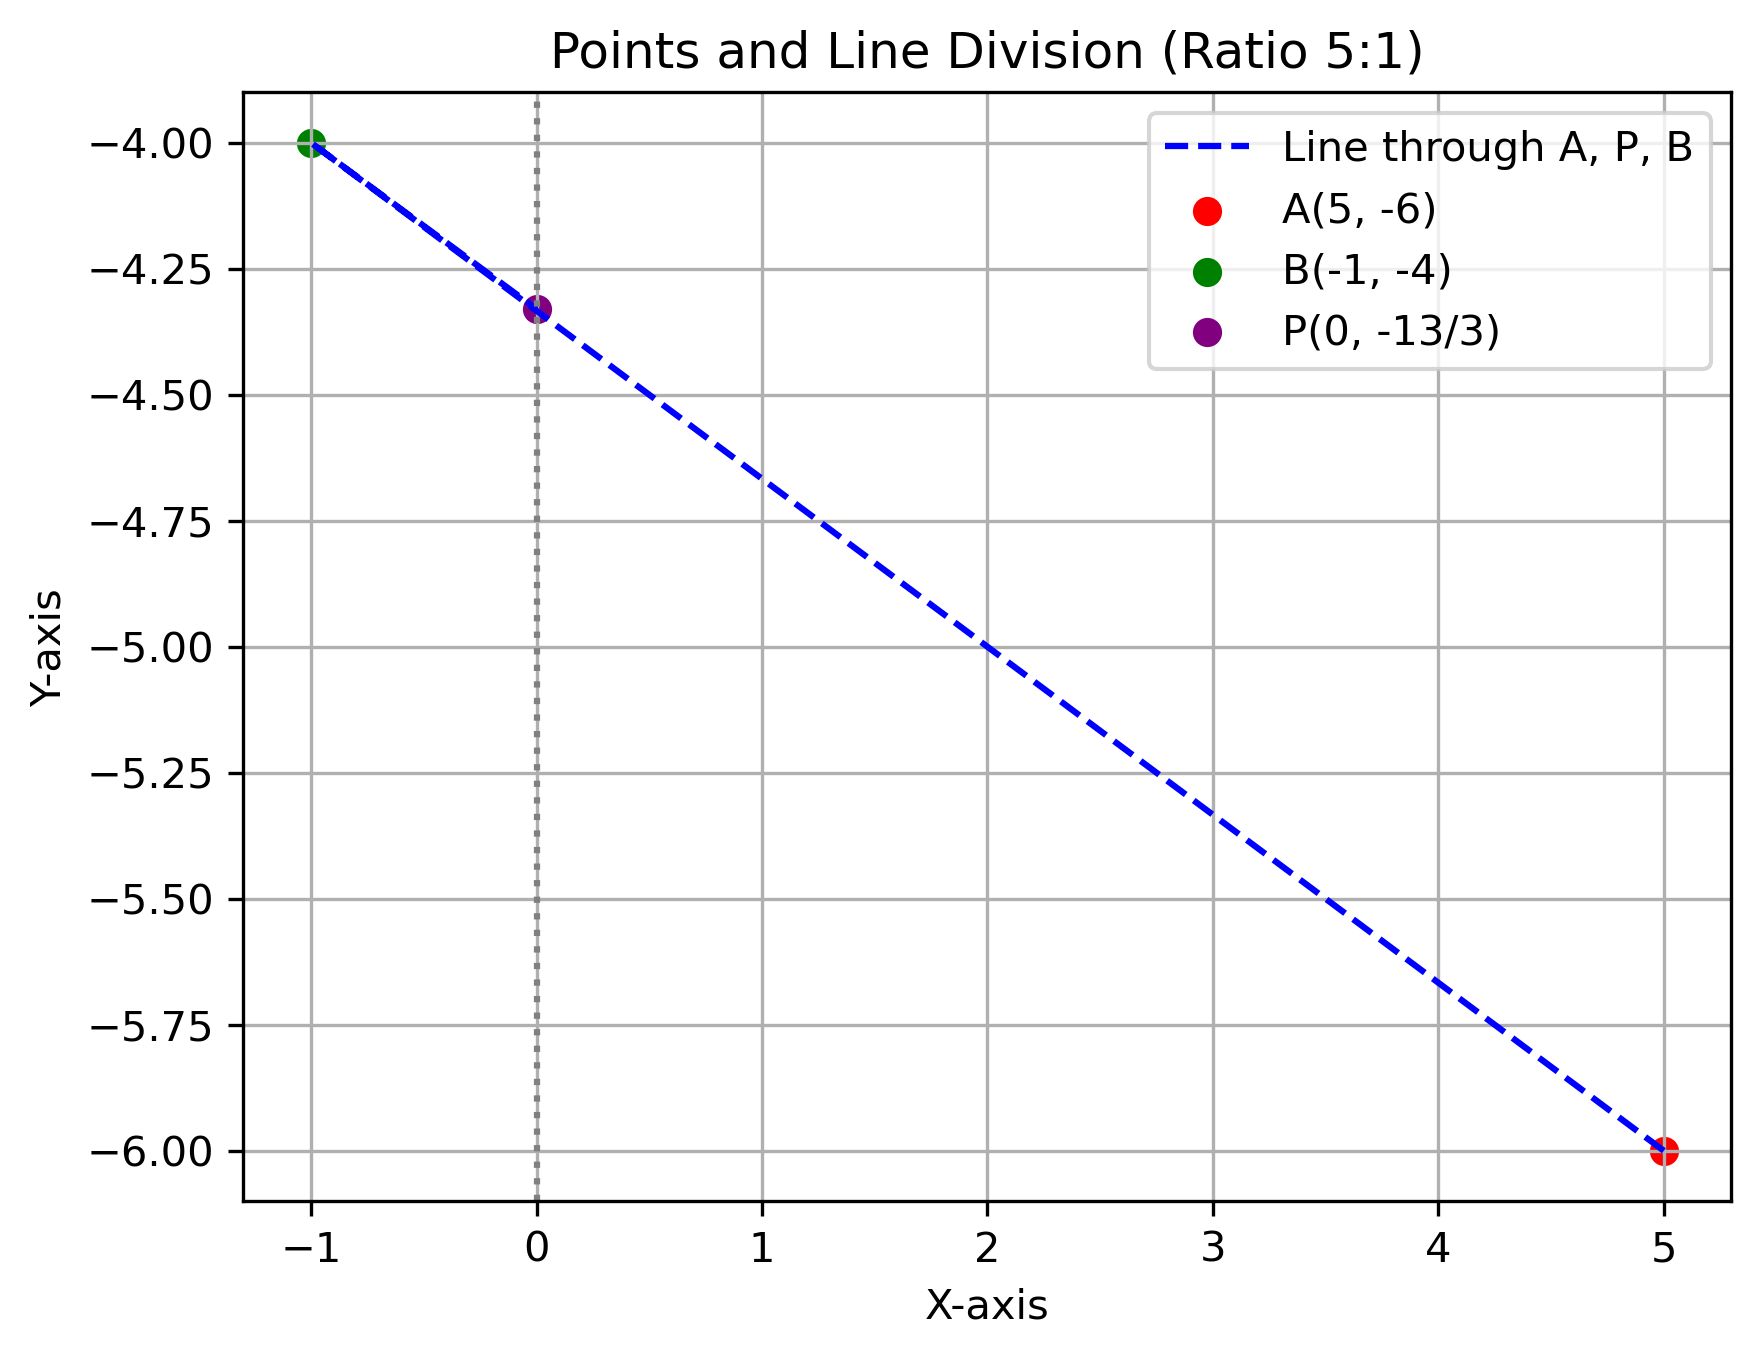
\includegraphics[width=0.5\columnwidth]{figs/fig1.png}
     \caption{}
     \label{fig:fig1}
 \end{figure}
\end{frame}

% ==================
\section{Conclusion}
\begin{frame}{Conclusion}
  The point $P(0,-\tfrac{13}{3})$ divides the line segment $AB$ in the ratio $5:1$.
\end{frame}

\end{document}
